\documentclass[../../General.tex]{subfiles}
\begin{document}


\section{Módulo de actuadores y controladores de potencia}

\subsection{Identificación y especificaciones nominales de los actuadores}

El sistema mecatrónico incorpora cinco actuadores dedicados a los diferentes grados de libertad del vehículo, cuyas especificaciones de placa determinan las exigencias de potencia para los circuitos de conmutación.

El actuador M1, destinado al ajuste angular de cabeceo de la plataforma de medición superior, corresponde a un motor paso a paso híbrido bipolar NEMA 17 (modelo  17HS19-2004S1) con dos fases, ángulo de paso de $1.8^\circ$, corriente nominal de $2.00\text{ A/fase}$, resistencia de devanado de $1.40\text{ }\Omega$, inductancia de $3.00\text{ mH}$ y torque de retención de $0.59\text{ N}\cdot\text{m}$.

El actuador M2, asignado a la elevación vertical del mecanismo de cuadrilátero articulado, consiste en un motor paso a paso híbrido bipolar NEMA 23 acoplado a una caja reductora planetaria integrada con relación de $4.29:1$ (modelo 23HS22-2804S-PG4). Este conjunto presenta una corriente nominal de $2.80\text{ A/fase}$, resistencia de $0.90\text{ }\Omega$, inductancia de $2.50\text{ mH}$, holgura angular inferior a $1.5^\circ$ y capacidad para entregar un torque continuo admisible de $20.0\text{ N}\cdot\text{m}$, con un ángulo de paso efectivo en el eje de salida de aproximadamente $0.4194^\circ$.

Los actuadores M3 y M4, encargados del mecanismo de viraje tipo Ackermann en las manguetas del eje frontal, son servomotores digitales de alto torque (modelo Dsservo RDS3225) provistos de piñonería metálica de cobre y aluminio con doble rodamiento de bolas. Estos componentes operan en un rango de voltaje de $4.8\text{ V}$ a $6.8\text{ V}$, entregando un torque de bloqueo de $2.40\text{ N}\cdot\text{m}$ a $6.8\text{ V}$ con una corriente de estancamiento de $2.3\text{ A}$ por unidad y un tiempo de respuesta de $0.13\text{ s}/60^\circ$.

El actuador M5, responsable de la tracción en el eje posterior, es un motorreductor de corriente directa (DC) con escobillas e imán permanente de $24\text{ V}$. Este incorpora una etapa de engranajes reductores para proporcionar bajas revoluciones con una potencia nominal de salida de $60\text{ W}$, corriente de trabajo continuo de $2.50\text{ A}$, corriente transitoria de arranque de $7.50\text{ A}$ y un torque nominal de salida de $15\text{ N}\cdot\text{m}$.

\subsection{Controlador para el mecanismo de orientación de la plataforma}

El mecanismo de cabeceo del sensor de irradiancia exige una alta suavidad de desplazamiento para impedir vibraciones que descalibren el piranómetro. Con este fin, se evalúan tres controladores de micropasos compactos para el actuador M1, cuyas características se contrastan en la Tabla \ref{tab:comp_driver_tilt}.

\begin{center}
    \footnotesize
    \begin{xltabular}{\textwidth}{|p{3.2cm}|>{\centering\arraybackslash}X|>{\centering\arraybackslash}X|>{\centering\arraybackslash}X|}
        \caption{Tabla comparativa de drivers de micropasos para el motor de orientación Tilt\label{tab:comp_driver_tilt}} \\
        \hline
        \rowcolor[HTML]{D9E1F2} \textbf{Especificación Técnica} & \textbf{Opción A (Trinamic TMC2209)} & \textbf{Opción B (A4988)} & \textbf{Opción C (DRV8825)} \\
        \hline
        \endfirsthead
        
        \multicolumn{4}{c}%
        {{\bfseries \tablename\ \thetable{} -- Continuación de la página anterior}} \\
        \hline
        \rowcolor[HTML]{D9E1F2} \textbf{Especificación Técnica} & \textbf{Opción A (Trinamic TMC2209)} & \textbf{Opción B (A4988)} & \textbf{Opción C (DRV8825)} \\
        \hline
        \endhead
        
        \hline
        \endfoot
        
        \hline
        \endlastfoot
        Corriente Eficaz y Máxima & 2.0 A eficaz y 2.8 A pico & 1.2 A eficaz y 2.0 A pico & 1.5 A eficaz y 2.2 A pico \\
        \hline
        Interpolación de Micropasos & Disponible hasta 256 micropasos & Sin interpolación interna & Sin interpolación interna \\
        \hline
        Modulación Silenciosa & Tecnología StealthChop2 & Chopper convencional ruidoso & Ruido audible a baja velocidad \\
        \hline
        Interfaz de Control & Señales de paso y dirección & Señales de paso y dirección & Señales de paso y dirección \\
        \hline
        Protección de Sobrecarga & Detección de pérdida de paso & Sin diagnóstico avanzado & Sin diagnóstico avanzado \\
        \hline
        Evaluación de Idoneidad & Seleccionado para la aplicación & Descartado por ruido mecánico & Descartado por vibraciones \\
        \hline
    \end{xltabular}
\end{center}

Se selecciona el controlador Trinamic TMC2209. Este circuito integra la tecnología de modulación StealthChop2 basada en control de voltaje, la cual erradica las resonancias acústicas. Los terminales de selección de microstep (MS1 y MS2) se configuran a nivel lógico alto conectándolos a la línea de $5.0\text{ V}$, fijando una resolución base de $1/16$ de paso que el interpolador interno (MicroPlyer) amplía de manera automática a $256$ micropasos homogéneos.

Para proteger la etapa de potencia ante voltajes inducidos por desaceleración rápida o frenado regenerativo, se dispone un diodo supresor de transitorios (TVS) unidireccional de $30\text{ V}$ en paralelo con un condensador electrolítico de $100\text{ }\mu\text{F}$ montado inmediatamente en las terminales de entrada de $24\text{ V}$. La corriente eficaz de trabajo ($I_{\text{RMS}}$) se calibra al $70\%$ del valor nominal del motor para mantener una temperatura de operación moderada, fijándose en $1.40\text{ A}_{\text{RMS}}$ ($1.98\text{ A}$ de pico). Empleando la resistencia de medición de corriente ($R_{\text{sense}}$) de $0.11\text{ }\Omega$ presente en el módulo, el voltaje de referencia analógico ($V_{\text{REF}}$) del potenciómetro de ajuste se gradúa exactamente en $1.98\text{ V}$.

\subsection{Controlador para el mecanismo de elevación del cuadrilátero}

El mecanismo articulado de elevación demanda sostener y desplazar la masa de la plataforma de instrumentación de forma estable. Se analizan tres dispositivos de potencia comerciales para el actuador M2, detallados en la Tabla \ref{tab:comp_driver_elevacion}.

\begin{center}
    \footnotesize
    \begin{xltabular}{\textwidth}{|p{3.2cm}|>{\centering\arraybackslash}X|>{\centering\arraybackslash}X|>{\centering\arraybackslash}X|}
        \caption{Tabla comparativa de drivers bipolares para el motor NEMA 23 del cuadrilátero articulado\label{tab:comp_driver_elevacion}} \\
        \hline
        \rowcolor[HTML]{D9E1F2} \textbf{Especificación Técnica} & \textbf{Opción A (Leadshine DM542)} & \textbf{Opción B (TB6600)} & \textbf{Opción C (DRV8825)} \\
        \hline
        \endfirsthead
        
        \multicolumn{4}{c}%
        {{\bfseries \tablename\ \thetable{} -- Continuación de la página anterior}} \\
        \hline
        \rowcolor[HTML]{D9E1F2} \textbf{Especificación Técnica} & \textbf{Opción A (Leadshine DM542)} & \textbf{Opción B (TB6600)} & \textbf{Opción C (DRV8825)} \\
        \hline
        \endhead
        
        \hline
        \endfoot
        
        \hline
        \endlastfoot
        Tensión de Operación & De 20.0 V a 50.0 V continuos & De 9.0 V a 40.0 V continuos & De 8.2 V a 45.0 V continuos \\
        \hline
        Corriente Ajustable Pico & De 1.0 A a 4.2 A por fase & De 0.5 A a 3.5 A por fase & De 0.5 A a 2.2 A por fase \\
        \hline
        Algoritmo de Conducción & Procesador digital antirresonancia & Chopper analógico convencional & Chopper analógico convencional \\
        \hline
        Aislamiento de Señales & Optoacopladores de alta velocidad & Optoacopladores estándar & Entradas lógicas directas \\
        \hline
        Rango de Micropasos & Desde medio paso hasta 128 micropasos & Desde paso completo a 32 pasos & Desde paso completo a 32 pasos \\
        \hline
        Chasis y Disipación & Gabinete de aluminio aletado & Carcasa con base metálica & Placa pequeña sin disipador \\
        \hline
        Evaluación de Idoneidad & Seleccionado para la aplicación & Descartado por vibraciones & Descartado por sobrecalentamiento \\
        \hline
    \end{xltabular}
\end{center}

Se selecciona el controlador industrial Leadshine DM542. El dispositivo cuenta con un procesador digital de señales (DSP) de 32 bits que implementa compensación de resonancia en lazo cerrado y entradas diferenciales optoacopladas que admiten niveles de $5.0\text{ V}$ en configuración de cátodo común, vinculando las señales de paso, dirección y habilitación a los terminales digitales correspondientes del microcontrolador.

La parametrización física se realiza mediante el bloque de interruptores DIP integrados. La corriente de fase se calibra en $2.84\text{ A}_{\text{pico}}$ ($2.03\text{ A}_{\text{RMS}}$), suministrando el torque nominal sin saturar el núcleo del motorreductor. El cuarto conmutador se configura en estado inactivo para habilitar la reducción automática de corriente al $50\%$ tras $1\text{ s}$ de inactividad motriz, atenuando la disipación térmica estática en un $75\%$. Los conmutadores de resolución se ajustan a $1/8$ de paso ($1600\text{ pulsos/rev}$ en el eje del motor), lo que conjugado con la reducción planetaria de $4.29:1$ entrega una resolución final de $0.0524^\circ/\text{pulso}$ en el eje de accionamiento del cuadrilátero. La alimentación se desacopla mediante un condensador electrolítico de $470\text{ }\mu\text{F}$ a $50\text{ V}$ ubicado en los bornes de potencia del módulo.

\begin{figure}[H]

	\captionsetup{justification=raggedright, singlelinecheck=false, labelsep=none}
	
	\caption[.]{} 
	
	\textit{.} \par\medskip
	
	\begin{minipage}{0.5\textwidth}
		\centering
		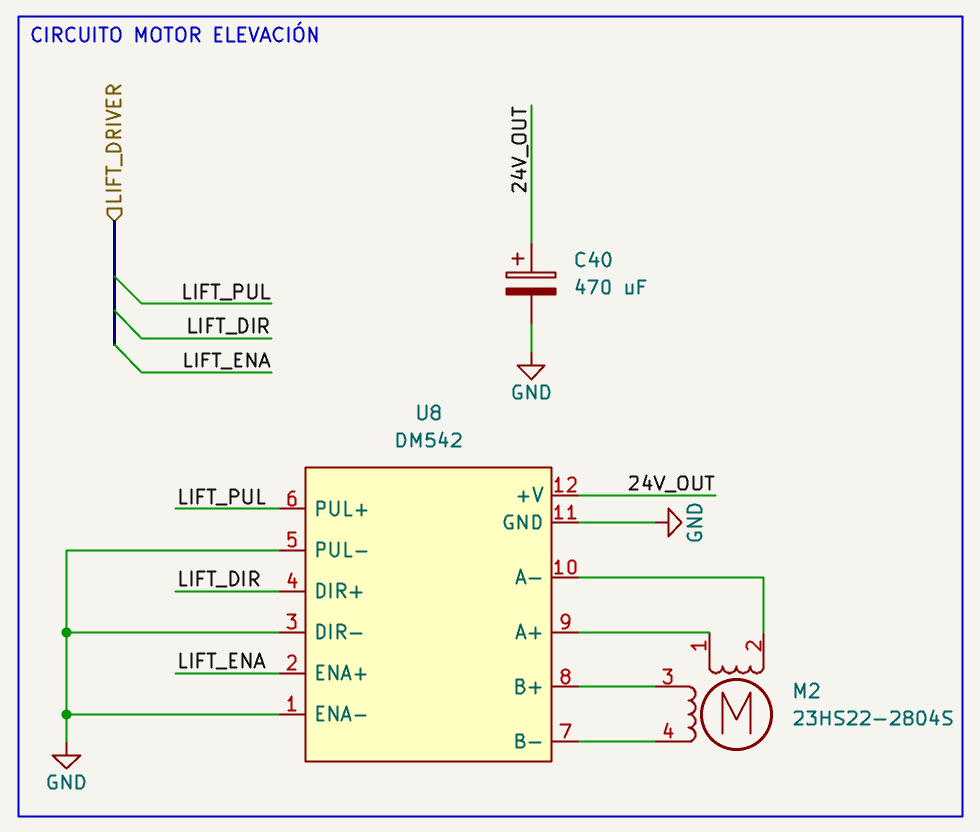
\includegraphics[width=\linewidth]{Recursos/Imagenes/ImagenesDisenoElectronico/MotorLift.png}
	\end{minipage}\hfill
	\begin{minipage}{0.5\textwidth}
		\centering
		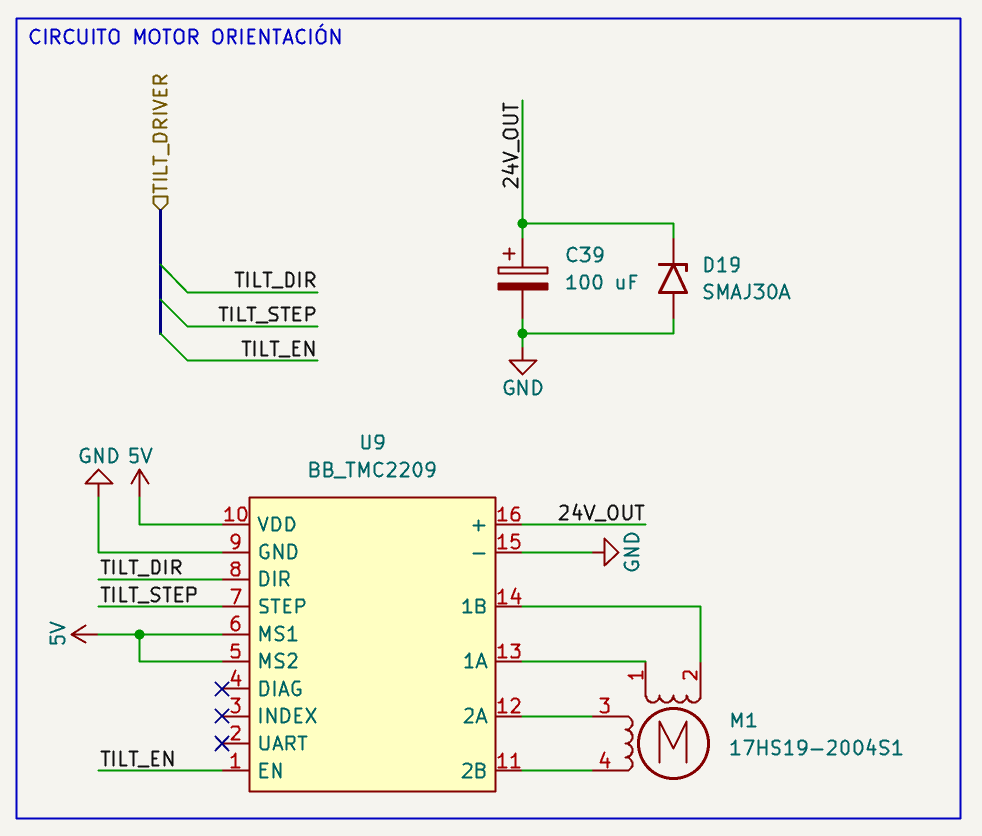
\includegraphics[width=\linewidth]{Recursos/Imagenes/ImagenesDisenoElectronico/MotorTilt.png}
	\end{minipage}
	\par\medskip
	
	\raggedright
	\footnotesize \textit{Nota.} Elaboración propia.
	\label{fig:MotorLiftTilt}
\end{figure}

\subsection{Controlador para el motorreductor de tracción}

El tren de rodadura posterior requiere gobierno sobre la velocidad y sentido de giro del motorreductor de corriente continua M5, empleando modulación por ancho de pulsos a frecuencias inaudibles para evitar zumbidos y desgastes prematuros. En la Tabla \ref{tab:comp_driver_traccion} se examinan tres módulos comerciales de puente completo.

\begin{center}
    \footnotesize
    \begin{xltabular}{\textwidth}{|p{3.2cm}|>{\centering\arraybackslash}X|>{\centering\arraybackslash}X|>{\centering\arraybackslash}X|}
        \caption{Tabla comparativa de controladores Puente H para el subsistema de tracción\label{tab:comp_driver_traccion}} \\
        \hline
        \rowcolor[HTML]{D9E1F2} \textbf{Especificación Técnica} & \textbf{Opción A (BTS7960)} & \textbf{Opción B (VNH5019)} & \textbf{Opción C (L298N Dual)} \\
        \hline
        \endfirsthead
        
        \multicolumn{4}{c}%
        {{\bfseries \tablename\ \thetable{} -- Continuación de la página anterior}} \\
        \hline
        \rowcolor[HTML]{D9E1F2} \textbf{Especificación Técnica} & \textbf{Opción A (BTS7960)} & \textbf{Opción B (VNH5019)} & \textbf{Opción C (L298N Dual)} \\
        \hline
        \endhead
        
        \hline
        \endfoot
        
        \hline
        \endlastfoot
        Tensión de Operación & De 6.0 V a 28.0 V continuos & De 6.0 V a 24.0 V continuos & De 5.0 V a 12.0 V continuos \\
        \hline
        Capacidad de Corriente & 43.0 A continuo y 60.0 A pico & 12.0 A continuo y 30.0 A pico & 2.0 A continuo y 3.0 A pico \\
        \hline
        Frecuencia Máxima de Conmutación & Hasta 25 kHz de frecuencia & Hasta 20 kHz de frecuencia & Menor a 10 kHz de frecuencia \\
        \hline
        Aislamiento Integrado & Aislamiento optoelectrónico & Sin aislamiento nativo & Sin aislamiento nativo \\
        \hline
        Resistencia en Conducción & 16 miliohmios por rama & 18 miliohmios por rama & Caída de voltaje mayor a 1.8 V \\
        \hline
        Protecciones Incorporadas & Térmica, sobrecorriente y subtensión & Térmica y sobrecorriente & Sin protecciones activas \\
        \hline
        Evaluación de Idoneidad & Seleccionado para la aplicación & Descartado por costo unitario & Descartado por capacidad eléctrica \\
        \hline
    \end{xltabular}
\end{center}

Se selecciona el módulo BTS7960, integrado por dos semicircuitos de potencia con transistores MOSFET de canal N y resistencia en conducción ($R_{\text{DS(on)}}$) de $16\text{ m}\Omega$. Esta capacidad otorga un margen de seguridad superior a diez veces respecto al régimen nominal continuo del motorreductor ($2.50\text{ A}$), manteniendo temperaturas de operación moderadas con el disipador metálico pasivo incorporado.

Las terminales de habilitación y modulación por ancho de pulso se conectan directamente a pines digitales y salidas de temporizador por hardware del microcontrolador, mientras que los pines de diagnóstico analógico de corriente se mantienen desconectados de acuerdo con la directiva de diseño. En paralelo con la entrada de fuerza se disponen un diodo supresor de transitorios (TVS) de $30\text{ V}$ y un condensador electrolítico de $470\mu\text{F}$ para amortiguar las corrientes regenerativas generadas durante desaceleraciones o paradas bruscas.

\subsection{Accionamiento y filtrado para los servomotores de dirección}

La orientación de las ruedas directrices frontales se ejecuta mediante los dos servomotores M3 y M4 acoplados al varillaje Ackermann. Al integrar cada unidad su propio microcontrolador interno, potenciómetro de retroalimentación y puente de transistores (puente H), no se requiere un controlador de potencia externo adicional.

Las líneas de comando de ambos servomotores se enlazan de forma directa con dos salidas de temporizador (PWM por hardware) del microcontrolador Arduino Mega 2560, el cual suministra trenes de pulsos periódicos a una frecuencia base de $50\text{ Hz}$ ($T = 20\text{ ms}$). El ancho de los pulsos modula continuamente entre $500\mu\text{s}$ para el tope angular extremo izquierdo y $2500\mu\text{s}$ para el tope derecho, situándose la posición neutra de avance en línea recta en $1500\mu\text{s}$. La potencia eléctrica se recibe de manera exclusiva desde la barra dedicada de $6.0\text{ V}$ provista por el convertidor reductor conmutado, cuyo banco de filtrado local de $940\mu\text{F}$ absorbe las transiciones de corriente asociadas a la corrección de rumbo sobre irregularidades del terreno.


\begin{figure}[H]

	\captionsetup{justification=raggedright, singlelinecheck=false, labelsep=none}
	
	\caption[.]{} 
	
	\textit{.} \par\medskip
	
	\begin{minipage}{0.5\textwidth}
		\centering
		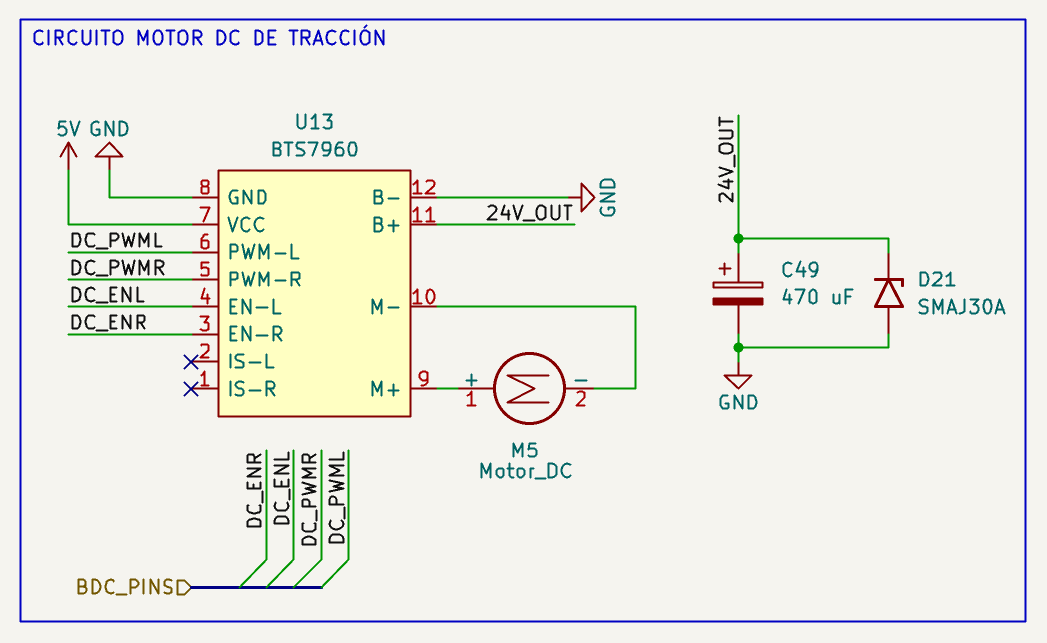
\includegraphics[width=\linewidth]{Recursos/Imagenes/ImagenesDisenoElectronico/DCMotor.png}
	\end{minipage}\hfill
	\begin{minipage}{0.5\textwidth}
		\centering
		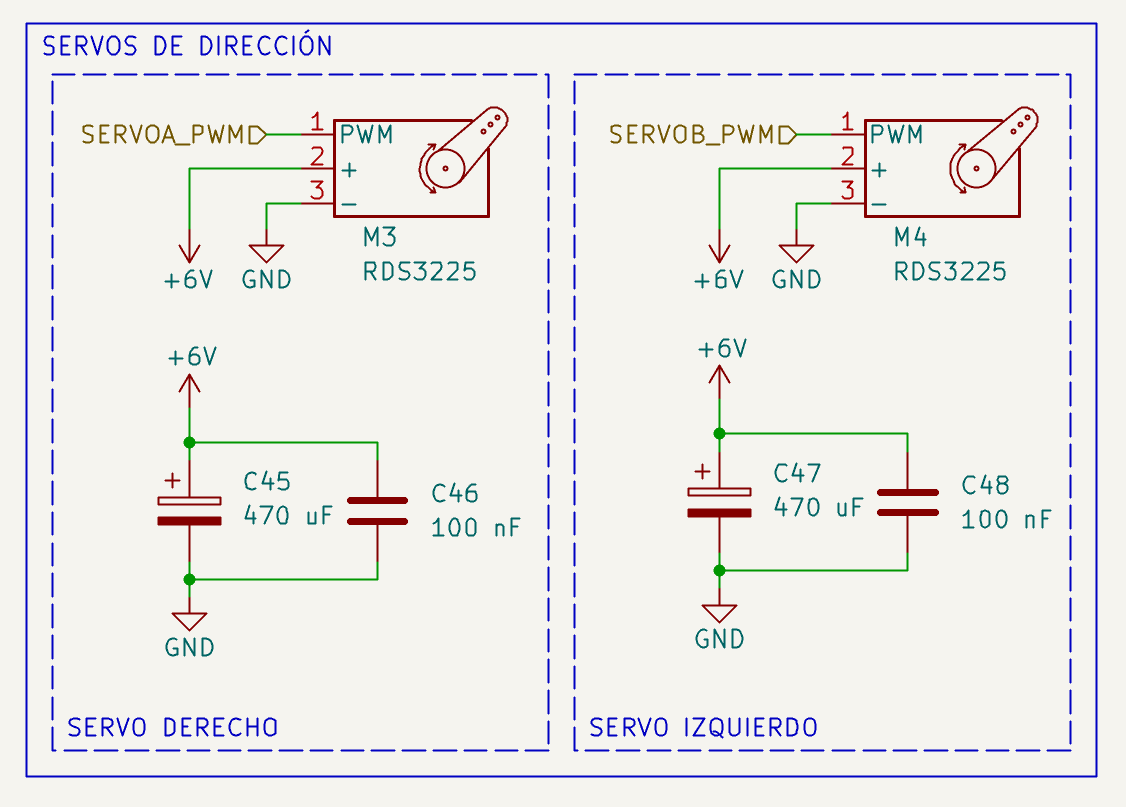
\includegraphics[width=\linewidth]{Recursos/Imagenes/ImagenesDisenoElectronico/ServoMotorCircuit.png}
	\end{minipage}
	\par\medskip
	
	\raggedright
	\footnotesize \textit{Nota.} Elaboración propia.
	\label{fig:DCServoMotor}
\end{figure}

\subsection{Análisis de demanda de corriente y regímenes transitorios en el bus de actuadores}

Debido a que los controladores de los motores paso a paso operan mediante fuentes conmutadas por modulación de corriente constante y el convertidor de los servomotores posee una alta eficiencia energética, la corriente demandada a la barra principal de $24\text{ V}$ es significativamente menor que la suma aritmética de las corrientes de fase de los devanados.

En régimen estacionario o de espera, con el motorreductor de tracción desactivado, el controlador TMC2209 en retención al $50\%$ consume $0.12\text{ A}$, el controlador DM542 con reducción activa demanda $0.30\text{ A}$ y los dos servomotores en posición fija extraen $0.02\text{ A}$, resultando en una corriente en reposo de $0.44\text{ A}$ que equivale a una potencia estática de $10.6\text{ W}$.

En condición de marcha ordinaria con inspección activa sobre pasillos solares, el motorreductor de tracción desplazando al robot demanda un promedio de $1.00\text{ A}$ a $24\text{ V}$, el actuador de elevación ejecutando correcciones suaves consume $0.85\text{ A}$, el actuador de orientación requiere $0.45\text{ A}$ y los servomotores frontales en corrección periódica consumen $0.25\text{ A}$, consolidando una corriente media de $2.55\text{ A}$ que representa una potencia activa de $61.2\text{ W}$.

En el escenario transitorio más severo, caracterizado por la aceleración simultánea de los mecanismos y una detención momentánea de la rueda trasera por bloqueo mecánico, el consumo instantáneo puede alcanzar $0.80\text{ A}$ en el actuador de orientación, $1.80\text{ A}$ en el de elevación, $1.45\text{ A}$ en los servomotores y $7.50\text{ A}$ durante el pico de arranque del motorreductor, totalizando una demanda instantánea de $11.55\text{ A}$. Esta magnitud es soportada sin interrupciones por el fusible térmico principal de $10\text{ A}$ (debido a su curva de disparo lento) y los contactos de $15\text{ A}$ del relé de aislamiento.


\end{document}